\chapter{Revisão Bibliográfica}
\label{cap:revisao_bibliografica}
\section{Sistemas Embarcados}
\label{sec:sis_embarcados}
Diferentemente dos computadores do dia-dia, ou seja, de propósito geral, em sistemas embarcados o software é acoplado à um hardware dedicado, sendo as funcionalidades implementadas de acordo com os requisitos e também com as características e particularidades de seus componentes físicos sendo utilizados. Sua principal característica é o fato de ser destinado a executar tarefas específicas \cite{li2003real}

Segundo \cite{cunha2013} a inteligência embarcada é uma tendência futura, cada vez mais inteligência será adicionada aos equipamentos do dia-a-dia, considera que um micro-ondas atual tem mais capacidade computacional do que tinha o projeto Apolo, que levou o homem a lua. Esta crescente utilização se dá basicamente pelo preço e consumo reduzido dos microcontroladores, além da grande flexibilidade ao atender os mais diversos problemas visto o vasto número de arquiteturas disponíveis: ARM, MIPS, Coldfire/68k, PowerPC, x86, PIC, 8051, Atmel AVR, Renesas H8, SH, V850, FR-V, M32R, Z80, Z8 e outras. Um contraste que atrai diversos desenvolvedores quando comparado com o número limitado de arquiteturas diponíveis para microprocessadores do mercado de computadores pessoais \cite{germano2011}.

A comunicação dos microcontroladores com o meio externo, segundo \cite{germano2011}, se dá pelos periféricos e o mais comuns são:
\begin{itemize}
\item Entrada de dados através de teclas, geralmente pelo de teclados feitos com varredura matricial;
\item \emph{Leds};
\item \emph{Display’s} de LCD, sendo os mais comuns os alfanuméricos como o HD44780;
\item Interface serial, por exemplo RS232 e I2C;
\item USB, \emph{Universal Serial Bus};
\item TCP/IP.
\end{itemize}

Como dito anteriormente, esses sistemas estão cada vez mais no dia-a-dia das pessoas e, claro, facilitando a vida delas, mas muitas vezes não são percebidos. E cada vez mais estão mais acessíveis podendo automatizar funções até mesmo dentro das próprias casas. %A Figura 

\section{Sistemas Embarcados de Tempo Real}
\label{sec:sis_embarcados_tempo_real}
O conceito Tempo Real vem da ideia básica em que é esperado que o software execute ou dê um retorno de sua execução até um limite de tempo bem definido. Normalmente pessoas assumem que tempo real significa "muito rápido", entretanto não é verdade, tempo real simplesmente significa "rápido o suficiente" no contexto de operação do sistema. Um exemplo é a ação do motor, pode-se dizer que é "rápida", pois o sistema deve tomar decisões como - fluxo de combustível, tempo da faísca - toda vez que o motor completa um ciclo.

Sistemas de tempo real são baseados em previsibilidade e, segundo \cite{farines2000sistemas}, essa previsibilidade de um sistema de tempo real é obtida quando independente de falhas, sobrecargas e variações de hardware, e assim é possível que seu comportamento seja antecipado antes de sua execução. Isso tem a finalidade de poder prever o funcionamento de um sistema de tempo real e garantir as suas restrições temporais, e para isso é necessário definir hipóteses em relação a carga e falhas em relação ao ambiente externo deste sistema \cite{farines2000sistemas}. 
Segundo \cite{mall2009real} os sistemas de tempo real são classificados em dois tipos:
\begin{itemize}
\item \emph{Soft Real Time Systems}: Sistemas não críticos de tempo real, onde a ocorrência de uma falha temporal é da mesma ordem de grandeza que os resultados em que o funcionamento está correto, exemplos: Máquina de lavar e portão eletrônico de uma casa;
\item \emph{Hard Real Time Systems}: Sistemas Críticos de Tempo Real, onde a ocorrência de uma falha temporal complicam, e muito, os resultados quando comparado com seu funcionamento correto, exemplos: sistema de controle de um avião e um sistema de controle de semáforos.
\end{itemize}

\section{Sistemas Embarcados Críticos}
\label{sec:sis_embarcados_critico}

Sistema Crítico é um sistema no qual a confiança é fundamental, ou melhor, a questão mais importante em seu desenvolvimento. Isso porque sistemas críticos, em caso de falha, podem causar consequências gravíssimas para os humanos, economia e outras áreas. Pode-se dizer que seus indicadores são: Disponibilidade, confiabilidade, segurança e proteção. E para que essa confiança seja alcançada deve-se evitar erros durante seu desenvolvimento e realizar diversos testes para que seja possível detectar e corrigir os erros que passarem de forma que seja possível limitar os danos causados por falhar operacionais \cite{sommerville2004software,feldmann2007survey,jordan2006standard}.

Segundo \cite{kopetz2011real} as classificações dos sistemas embarcados críticos podem ser:
\begin{itemize}
\item \emph{Fail Safe}: Classificação para sistemas onde o estado seguro pode ser atingido em caso de falha, como por exemplo, esgotar a bateria de uma bomba de insulina;
\item \emph{Fail Operational}: Classificação para sistemas que em caso de falhas ainda são capazes de fornecer algum tipo de serviço, mesmo que mínimo. Um exemplo é um sistema de controle de voo que, mesmo em caso de falha, é capaz de fornecer serviços e ser seguro.
\end{itemize}

\section{Microcontrolador}
\label{sec:microcontrolador}

Segundo \cite{ganssle1999art}, o microcontrolador é a parte mais importante de um sistema embarcado e sua principal diferença quando comparada com um microprocessador é o fato de ser um sistema computacional completo que integra todos as principais partes da arquitetura de Von Neumann em um único componente, as partes citadas são:
\begin{itemize}
\item CPU: \emph{Central Processor Unit};
\item Memória RAM: \emph{Random Access Memory};
\item Portas I/O: Portas de entrada e saída.
\end{itemize}

Além de ser composto por temporizadores, memória ROM (\emph{Read Only Memory}), conversor AD, analógico – digital, e DA, digital – analógico.
Comparados com microprocessadores, os microcotroladores possuem consumo e \emph{clock}, processamento, reduzidos, isso devido ao fato que o primeiro é destinado a tarefas que necessita uma alta capacidade de processamento como, por exemplo, os microprocessadores do nosso PC do dia-a-dia. Por padrão, os microprocessadores são utilizados em situações que os requisitos são abrangentes, com entradas e saída variadas como: sensores, atuadores e periféricos de comunicação \cite{lee2011introduction}.

\section{PIC18F452}
O PIC18F452 é um microcontrolador fabricado pela empresa \emph{Microchip Technology}. Possui tecnologia CMOS, como consequência tem um consumo baixíssimo, possui memória do tipo FLASH, um grande facilidade para desenvolvimento de protótipos, uma vez que para apagá-la não é preciso utilizar luz ultravioleta como em versões antigas, utilizavam memória EEPROM. Abaixo seguem as principais características desse microcontrolador:

\begin{itemize}
\item Microcontrolador de 40 Pinos;
\item Memória de programa FLASH de 32Kbytes;
\item Memória RAM de 1536 bytes;
\item Memória EEPROM de 256 bytes;
\item Processamento de até 10MIPS;
\item Quatro \emph{timers}, ou temporizadores, internos – um de 8 bits e 3 de 16 bits – TIMER0, TIMER1, TIMER2 e TIMER3;
\item 2 canais capture/compare/PWM – Módulo CCP;
\item Módulo \emph{Master Synchronous Serial Port} (MSSP);
\item \emph{Unhaced Usart;}
\item 8 canais A/D de 10 bits;
\item Detector de baixa voltagem programável;
\item Permite até 100.000 ciclos de escrita e leitura na memória FLASH;
\item Permite 1.000.000 ciclos de escrita e leitura na memória EEPROM.
\item Retenção de dados na FLASH por 40 anos;
\item \emph{Watchdog timer} com oscilador próprio e programável;
\item Três pinos de interrupções externas: INT0, INT1 e INT2
\end{itemize}

A Figura \ref{fig:pic} representa uma imagem do microcontrolador.

\begin{figure}[htp]
	\centering
	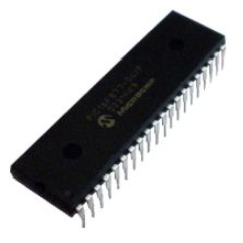
\includegraphics[scale=1]{images/pic.png}
	\caption{PIC18F452}	
	\label{fig:pic}	
\end{figure}

\newpage 
\subsection{Estrutura Interna}
A Figura \ref{fig:estuturapic} ilustra como é a estrutura interna do microcontrolador:

\begin{figure}[htp]
	\centering
	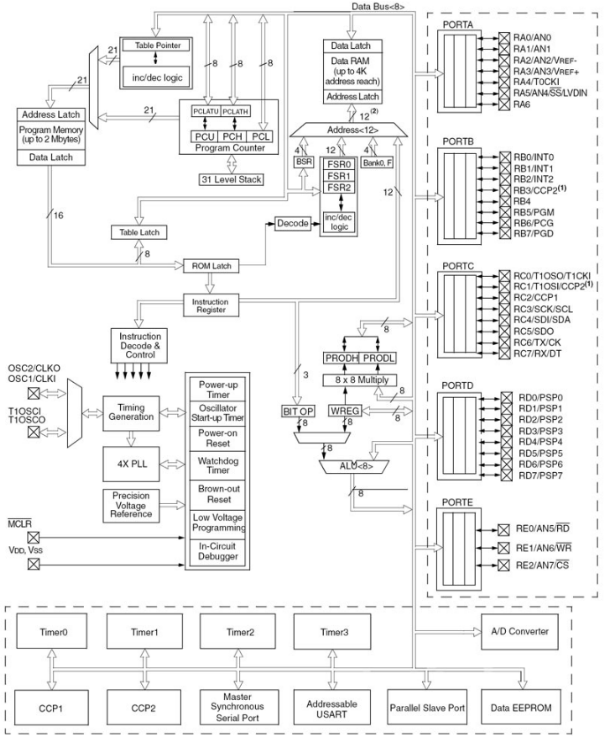
\includegraphics[scale=0.6]{images/estrutura_pic.png}
	\caption{Estrutura Interna PIC18F452}	
	\label{fig:estuturapic}	
\end{figure}

\newpage 
\subsection{DESCRIÇÃO DOS PINOS}
Dos 40 pinos desse microcontrolador 34 são pinos I/O, entrada e saída, divididos em 5 "PORT". A Figura \ref{fig:pinospic} representa uma relação dos pinos do microcontrolador.

\begin{figure}[htp]
	\centering
	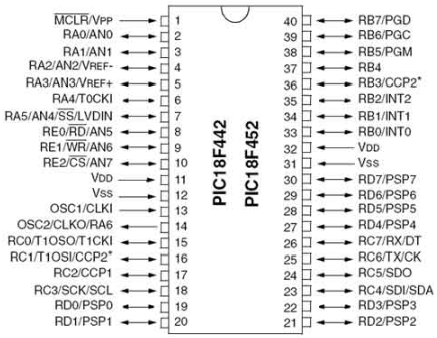
\includegraphics[scale=0.6]{images/pinos_pic.png}
	\caption{Pinos PIC18F452}	
	\label{fig:pinospic}	
\end{figure}

A divisão dos pinos I/O citada é da seguinte maneira:

\begin{itemize}
\item PORTA: São 7 pinos nomeados de RA0 a RA6. Podem ser utilizados como I/O geral ou conversor A/D, essa segundo opção tem exceção o pino RA4. Além de possuir a opção LVD, detecção de baixa tensão;
\item PORTB: São 8 pinos nomeados de RB0 a RB7. Podem ser utilizados para I/O geral e, além disso, pode-se trabalhar com três interrupções externas, módulo CCP, pinos de gravação e debug;
\item PORTC: São 8 pinos nomeados de RC0 a RC7. Podem ser utilizados para I/O geral, saída do oscilador do \emph{timer}, módulo CCP, Clock e data(dados) para os modos SPI, I2C e UART;
\item PORTD: São 8 pinos nomeados de RD0 a RD7. Podem ser utilizados para I/O geral ou como PSP para ter saída TTL, para interfaceamento com microprocessadores, por exemplo;
\item PORTE: São 3 pinos nomeados de RE0 a RE2. Podem ser utilizados para I/O geral ou pinos de controle de acesso.
\end{itemize}

\section{Sensores}
Segundo \cite{transdutores2004usp}, transdutores são equipamentos que transformam informações, ou seja, transformam um tipo de sinal em outro para permitir medições de grandezas, controles de outros equipamentos, entre outras formas de transformação. A definição de sensor pode ser a de um transdutor capaz de alterar sua característica física interna em resposta à um fenômeno físico externo. Além disso, existem sensores considerados de operação indireta que são os quais alteram suas propriedades como capacitância, resistência, ou, até mesmo, sua indutância, sob ação de algum gradeza ou evento externo \cite{rosario2006principios}. 

Segundo \cite{nomadusp2014}, os sensores são largamente utilizados na medicina, indústria, robótica, além de outras aplicações. Considerando que o sinal é sempre uma forma de energia, os sensores podem ser classificados em função da energia que é capaz de detectar, como:

\begin{itemize}
\item Sensores de luz: células solares, fotodíodos, fototransistores, tubos fotoelétricos, e outros;
\item Sensores de som: microfones e hidrofone;
\item Sensores de temperatura: termômetros e termopares;
\item Sensores de resistência elétricas: ohmímetro. 
\item Outros;
\end{itemize}

\subsection{Sensores Biológicos}
Segundo \cite{nomadusp2014}, os sensores citados anteriormente são corretamente chamados de sensores artificiais. Isto devido ao fato de existir sensores naturais ou biológicos, já que todos os organismos vivos possuem sensores capazes de agir da mesma forma que os artificias. Esses sensores biológicos são células especializadas, sensíveis a:

\begin{itemize}
\item Luz, movimento, temperatura, vibração, pressão, campos eléctricos, som, e outros aspectos físicos do ambiente;
\item Grande variedade de moléculas ambientais, incluindo toxinas e nutrientes;
\item Aspectos metabólicos, tais como os níveis de glicose e oxigênio;
\item Até mesmo as diferenças entre proteínas do ambiente externo e do próprio organismo.
\end{itemize}

Esses sensores artificiais que imitam sensores biológicos, utilizando componentes biológicos, são chamados biossensores.

\subsection{Atuadores}
Segundo \cite{chironis1991mechanisms}, dispositivos considerados atuadores são aqueles que transformam uma forma de energia em outra, causando mudanças no ambiente em que estão atuando, ou seja, de acordo com sinais, ou impulsos, recebidos realizam ações capazes de alterar as grandezas físicas do ambiente em questão. Eles são capazes de converter energias como: energia elétrica, hidráulica e pneumática em energia mecânica. Segue exemplos de alguns tipos de atuadores:

\begin{itemize}
\item Atuadores eletromagnéticos: São os motores elétricos como motores de passos, servos;
\item Atuadores hidráulicos: Utilizam um fluido submetido a uma pressão para movimentar um braço, são utilizados em robô que operam grandes cargas;
\item Atuadores pneumáticos: Utilizam um gás submetido a uma pressão para movimentar o braço, possuem menor custo que os hidráulicos, sendo utilizados em robôs de menor porte;
\end{itemize}

\subsection{Motor de Passo}
Motor de passo é um dispositivo eletromecânico. Sua principal propriedade é sua habilidade de transformar pulsos elétricos em movimentos, que são precisamente incrementados na posição do rotor e são denominados "passos". Esse tipo de motor é caracterizado como máquina duplamente saliente, significando que possui dentes, compostos por matérias magnéticos nas duas partes que o compõe: A parte imóvel chamada estator e a móvel rotor \cite{demotor, acarnley2002stepping}.

Seu uso é interessante em situações em que precisão nos movimentos é necessária. Isso porque com ele é possível controlar: ângulo de rotação, velocidade, posição e sincronismo. Suas vantagens não são seu torque nem a capacidade de gerar movimentos de alta velocidade, mas sim a precisão em seus movimentos. Devido a essas características esse tipo de motor é amplamente utilizado em: câmeras de vídeo, robôs, brinquedos, \emph{scanners}, impressoras, entre outros \cite{demotor}.

De forma simples o funcionamento de um motor de passo consiste no uso de materiais magnéticos, ou solenoides, como dito anteriormente, alinhados dois a dois, representando os polos norte e sul, que quando energizados atraem o rotor fazendo-o se alinhar as partes energizadas do estator, causando assim um pequeno movimento: o passo. Sua velocidade e sentido estão diretamente relacionados à forma com que os solenoides são acionados, o primeiro com a frequência e o segundo a ordem de acionamento \cite{demotor, acarnley2002stepping}.

\subsection{LCD - \emph{Liquid Crystal Display}}
Um \emph{display} de cristal líquido, LCD, é utilizado para exibir informações como texto, imagens e vídeos. É composto por um painel fino e, segundo \cite{lcd1996unicamp}, é um componente, considerado interface de saída, muito utilizados em conjunto com microcontroladores. Exemplos de uso são: \emph{cockpit} de aeronaves, \emph{displays} em computadores de bordo de automóveis, dispositivos de jogos, relógios, calculadoras e outros.

Pode-se classificar os módulos de LCD em: exibição gráfica e exibição de caractere. Os módulos gráficos são encontrados com resoluções de 122x32, 128x64, 240x64 e 240x128 pixel, possuindo, geralmente, 20 pinos para conexão. Já os modelos comuns, tipo caractere, tem sua especificação em função dos números de linhas e colunas.